\begin{figure*}[t!]
\begin{tikzpicture}
\node[inner sep=0pt] (taxonomy) at (0,0) {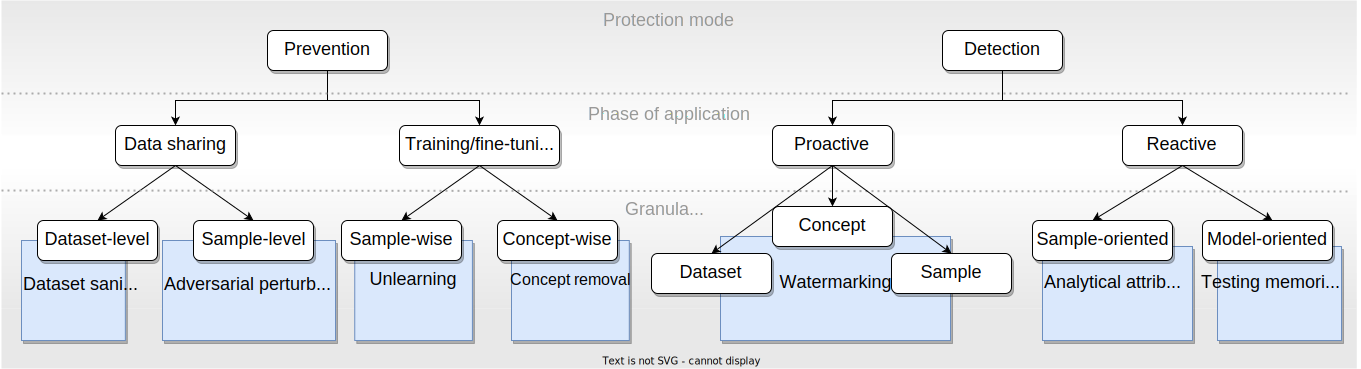
\includegraphics[width=\linewidth]{figures/taxonomy.drawio.pdf}};
% todo remove -- orientation
% \filldraw (0,0) circle (1pt);

% dataset sanitisation
\node[] (sanitisation1) at (-6.76,-0.63) {\tiny \cite{carlini_extracting_2023}};

%adversarial perturbations:
\node[] (adv1) at (-6.3,-1.60) {\tiny \cite{shan_glaze_2023,liang_adversarial_2023,liang_mist_2023,ye_duaw_2023,zhao_unlearnable_2023}};
\node[] (adv2) at (-6.32,-1.85) {\tiny \cite{chen_editshield_2023,salman_raising_2023,shan_prompt-specific_2023,zheng_understanding_2023}};
\node[] (adv3) at (-6.80,-2.1) {\tiny \cite{van_le_anti-dreambooth_2023,liu_toward_2023}};

% sanitisation
\node[] (sanitisation2) at (-4.52,-1.15) {\tiny\cite{somepalli_understanding_2023,li_mitigate_2024}};

% concept removal
\node[] (concept1) at (-3.25,-0.95) {\tiny\cite{kong_data_2023,schramowski_safe_2023,gandikota_erasing_2023}};
\node[] (concept2) at (-3.16,-1.2){\tiny\cite{gandikota_unified_2024,kumari_ablating_2023,zhang_forget-me-not_2023}};
\node[] (concept3) at (-3.40,-1.45){\tiny\cite{eldan_whos_2023,liu_rethinking_2024}};

% prompt modification
\node[] (prompt1) at (-1.65, -1.15) {\tiny\cite{somepalli_understanding_2023,noauthor_openai_2023}};
\node[] (prompt2) at (-1.6, -1.40) {\tiny\cite{hanu_detoxify_2020}};

% watermarking
% dataset-wise
\node[] (wm_dataset) at (1.0, -1.05) {\tiny\cite{cui_diffusionshield_2023}};
% sample-wise
\node[] (wm_sample1) at (2.65, -1.05) {\tiny\cite{zhang_editguard_2023,hayes_generating_2017,ma_generative_2023}};
\node[] (wm_sample2) at (2.65, -1.30) {\tiny\cite{cui_ft-shield_2023,tan_somewhat_2023,liu_detecting_2024}};
% concept-wise
\node[] (wm_concept) at (2.05,-0.50) {\tiny\cite{feng_catch_2023}};

% analytical attribution
\node[] (analytical_attr) at (5.03, -0.95) {\tiny\cite{somepalli_diffusion_2022,carlini_extracting_2023,wang_evaluating_2023,dai_training_2023}};

% testing memorisation 
\node[] (testing) at (6.85, -1.2) {\tiny\cite{carlini_secret_2019,tsai_ring--bell_2023,vyas_provable_2023}};

\end{tikzpicture}
\caption{Taxonomy of the IP protection methods for training data in GAI.}
\label{fig:taxonomy}
\end{figure*}
